\section{Matched Causal and Conformance Evaluation}

\subsection{Evaluation questions and evidence hierarchy}

The evaluation asks whether accepted runtime evidence can change receiver-local authorization before a harmful agent action, whether the single-environment reference path preserves receiver authority, whether timing changes the effect of evidence, and whether validation provides selective value beyond an arrival-triggered guard. The evidence hierarchy separates trace generation from enforcement causality. The deterministic study supplies the primary matched causal comparison. Credentialed live execution supplies a bounded cohort of agent-action traces. Strict replay fixes those traces while varying delivery. Single-environment reference-path arms exercise federation and gateway composition. The validation-value study, governed by a sealed pre-analysis plan, tests binding and receiver validation without live-model sampling; its hostile-peer and correlation tables are computed from declared formulas, not measured. Separately rooted post-denial substitution and independent-warning studies then test frozen branches and an externally authored warning population. Table~\ref{tab:units} defines the accounting units used below.

\begin{table*}[t]\centering\scriptsize
\caption{Units of analysis and accounting. Counts are not interchangeable across rows.}
\begin{tabular}{@{}p{0.16\textwidth}@{\hspace{0.35em}}p{0.28\textwidth}@{\hspace{0.35em}}p{0.46\textwidth}@{}}\toprule
Unit & Definition & Use in this paper \\ \midrule
Strict pair & One input-equivalent A1/A2 comparison with the same frozen local policy and action schedule & Primary deterministic causal comparison \\
Trace & One captured model-generated action sequence & Live cohort and frozen replay input \\
Replay treatment & One frozen trace evaluated at one action-relative context-delivery placement & Timing and availability accounting \\
Single-environment reference-path arm & One complete source-relay-evaluator-gateway execution in one reference environment & Gateway composition and authority provenance \\
Gateway call & One authorization request for an action opportunity & Harmful and benign forwarded or blocked outcomes \\
Signed exchange & One signed context transfer from \texttt{tcopd}-A to \texttt{tcopd}-B & Relay composition accounting \\
Validation episode & One credential-free mixed-action test case per condition & C0--C3 validation-value cohort \\ \bottomrule
\end{tabular}\label{tab:units}\end{table*}


\subsection{Deterministic matched design}

The deterministic evaluation compares isolated capable local observers (A1) against the same receiver configuration with accepted imported runtime evidence (A2). It holds local facts, local policy, frozen strategy, agent-action inputs, and action schedule fixed. The causal change is whether accepted evidence becomes available to Domain B. The synthetic scenarios and receiver strategy are constructed to test whether accepted evidence changes authorization under this matrix; the result is a causal conformance result, not an operational prevention estimate. For each pair, the evaluation records input equivalence, action-relative warning margin, local decision change, harmful-agent-action difference, and outcome direction.

For containment-first, the study includes \DeterministicPairs{} strict input-equivalent pairs. Imported context changes \DeterministicImproved{} outcomes and leaves \DeterministicUnchanged{} unchanged. Under strict matched replay, \DeterministicActionsPrevented{} harmful actions forwarded without context changed to blocked with matched TCOP context, reducing harmful calls from \DeterministicBaselineHarmfulCalls{} to \DeterministicTreatmentHarmfulCalls{}. Because containment-first can only add a restriction to the reported harmful-action measure, \DeterministicWorsened{} worsened pairs is a monotonicity check, not a surprising comparative result. Figure~\ref{fig:deterministic} shows the unchanged population rather than presenting only improved pairs.

The three residual harmful calls are the three strict resilience rows with no imported context or later harmful opportunity recorded. They are unchanged rather than late-warning failures, so the study does not attribute them to TCOP.

\begin{figure}[t]
\centering
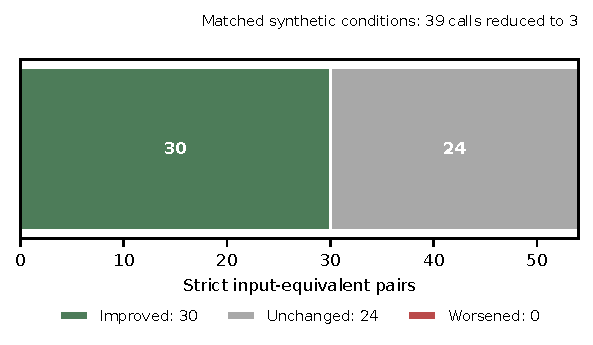
\includegraphics[width=\columnwidth]{deterministic-outcomes}
\caption{Deterministic strict-pair outcomes. The full matched population includes improved and unchanged pairs. The zero worsened count follows from the containment-first monotonicity of the reported harmful-action measure.}
\label{fig:deterministic}
\end{figure}

\begin{table}[t]\centering\small
\caption{Strict deterministic containment-first comparison. Balanced and utility configurations with unmatched local policies are excluded.}
\begin{tabular}{lr}\toprule
Metric & Value \\ \midrule
Strict input-equivalent pairs & \DeterministicPairs \\
Improved / unchanged / worsened & \DeterministicImproved / \DeterministicUnchanged / \DeterministicWorsened \\
Baseline / treatment harmful calls & \DeterministicBaselineHarmfulCalls / \DeterministicTreatmentHarmfulCalls \\
Harmful calls prevented & \DeterministicActionsPrevented/\DeterministicBaselineHarmfulCalls \\
Unmatched-policy exclusions & \DeterministicExcludedPairs \\ \bottomrule
\end{tabular}\label{tab:deterministic}\end{table}


\subsection{Admission rules and central control}

The study excludes \DeterministicExcludedPairs{} candidate balanced and utility comparisons from A1/A2 causal inference because their receiver-local policies differ. The exclusion ledger retains their inputs and the mismatch reason. This admission rule protects the question of whether imported context changed an outcome under the same local policy.

A fact-equivalent central audit holds exportable facts fixed while placing decision authority or an outage dependency in a central path. Across \CentralAuditCells{} audited cells, it records \CentralRegressions{} regressions: \CentralAuthorityRegressions{} associated with authority placement and \CentralOutageRegressions{} with central outage; \CentralNoRegression{} cells show no regression. It identifies dependencies of this construction, rather than serving as a general benchmark of centralized defense.

\subsection{Validation value beyond arrival}\label{sec:context-blanket}

The validation-value study holds receiver enforcement, action order, local facts, and warning arrival fixed across Local Only (C0), Arrival Default Allow (C1-allow), Arrival Guard (C1-class), Exact Binding (C2), and Standing Guard (C3). The study follows a sealed pre-analysis plan. The arrival conditions receive a valid-arrival token and a time-to-live. Exact Binding additionally evaluates issuer, signature, version, freshness, receipt, subject, resource namespace, capability class, scope, and receiver-local authorization state.

Table~\ref{tab:validation-value} reports the entire \ValidationEpisodes{}-episode mixed-action cohort. Arrival Default Allow forwards every action, showing that arrival by itself is not a containment policy. Standing Guard establishes the standing-restriction endpoint. Its complete harmful blocking comes with complete benign constraint.

Across the full cohort, Arrival Guard blocks \COneClassHarmfulBlocked{} of \ValidationEpisodes{} harmful actions and constrains \COneClassBenignConstrained{} of \ValidationEpisodes{} benign actions. Exact Binding blocks \CTwoHarmfulBlocked{} of \ValidationEpisodes{} harmful actions and constrains \CTwoBenignConstrained{} of \ValidationEpisodes{} benign actions. Within the accepted, binding-matched harmful subset, Arrival Guard and Exact Binding each block \COneClassMatchingBlocked{} of \MatchingHarmfulActions{} matching harmful actions. The additional Arrival Guard blocks occur under wrong-subject, wrong-resource, wrong-receipt, expired, replayed, and semantic-smuggling warning controls, which Exact Binding rejects. This is the measured selectivity result, not evidence that Exact Binding is a broader class guard.

\begin{table}[t]\centering\scriptsize
\caption{Mixed-action validation-value cohort governed by a sealed pre-analysis plan. Full-cohort harmful counts include mismatched-warning controls; the accepted binding-matched subset is reported separately in the text.}
\begin{tabular}{@{}p{0.43\columnwidth}rr@{}}\toprule
Condition & \shortstack{Harmful\\blocked} & \shortstack{Benign\\constrained} \\ \midrule
Local Only (C0) & \CZeroHarmfulBlocked/\ValidationEpisodes & \CZeroBenignConstrained/\ValidationEpisodes \\
Arrival Default Allow (C1-allow) & \COneAllowHarmfulBlocked/\ValidationEpisodes & \COneAllowBenignConstrained/\ValidationEpisodes \\
Arrival Guard (C1-class) & \COneClassHarmfulBlocked/\ValidationEpisodes & \COneClassBenignConstrained/\ValidationEpisodes \\
Exact Binding (C2) & \CTwoHarmfulBlocked/\ValidationEpisodes & \CTwoBenignConstrained/\ValidationEpisodes \\
Standing Guard (C3) & \CThreeHarmfulBlocked/\ValidationEpisodes & \CThreeBenignConstrained/\ValidationEpisodes \\ \bottomrule
\end{tabular}\label{tab:validation-value}\end{table}


\subsection{Correlation under ambiguity}

Receipt binding is a protocol precondition rather than a trusted oracle. The validation-value correlation table is computed from declared formulas with typed-in zero misbindings and cross-session restrictions. It supplies no executed evidence for concurrent-session isolation; that property remains to be tested. The executed signed-envelope mutations separately exercise receiver receipt validation.

\begin{table}[t]\centering\scriptsize
\caption{Validation-value evidence: executed receiver mutations and formula-computed illustrations.}
\begin{tabular}{@{}p{0.34\columnwidth}@{\hspace{0.4em}}p{0.57\columnwidth}@{}}\toprule
Check & Result \\ \midrule
Valid hostile-peer burst & Formula-computed illustration; no executed burst evidence. \\
Receipt correlation ambiguity & Formula-computed illustration with typed-in zeros; no measured correlation result. \\
Receiver-validator mutations & \ValidatorMutationCases{} mutations cover signature, issuer, version, receipt, expiry, and replay faults; action-like remote fields are retained as evidence and ignored for enforcement. \\ \bottomrule
\end{tabular}\label{tab:protocol-assurance}\end{table}


\subsection{Result interpretation}

An improved pair means that accepted runtime evidence changed a receiver-local outcome for the evaluated harmful-agent-action measure. An unchanged pair is an observed result: it includes actions that had already completed, evidence that was not actionable for a particular opportunity, and cells where the matched baseline produced the same local outcome. Availability is evaluated separately, so a harmful-action aggregate is not read as an unqualified benefit claim. In particular, this matched design establishes a receiver-path causal and conformance result, not an estimate of post-denial behavior prevalence or deployment effectiveness.
